\section{Autoregressive models}
\textbf{Goal} Density estim \(p({x}) = \prod_{i} p({x}_{i} | {x}_{<i})\).

\subsection*{Fully Visible Sigmoid Belief Networks}

Tabular approach needs \(2^{L}\) states not acceptable, replace with regression \(f_{i}(x_{1:i-1})= \sigma(\alpha_{0}^{i}+\sum_{j=1}^{i-1}\alpha_{j}^{i} x_{j})\),\\ \(p_{\theta_{i}}(x_{i} | x_{<i})=\operatorname{Ber}(f(x_{1:i-1}))\).


\subsection*{Neural Autoreg Density Estim (NADE)}
Extend FVSBN with NN, \({h}_{i}=\sigma({b}+{W}_{<i} {x}_{<i}),\) output \( \hat{x}_{i}=\sigma(c_{i}+V_{i} \mathbf{h}^{({i})})\).
Note: \(({b}+{W}_{\leq i} {x}_{\leq i})-({b}+{W}_{<i}{x}_{<i})={W}_{i}{x}_{i}\).

Train w/ NLL \(\sum_{t=1, i=1}^{T, D}  \ln p(x_{i}^{(t)} | x_{<i}^{(t)})\). Ground truth fed in conditional term for higher accuracy.

\textbf{Pros}: (1) Comput cost \(O(TD)\). (2) second-order optim OK (3) Reals and multinomials OK. (4) Random Order works fine.

\textbf{Variant}:
(1) Reals (RNADE) conds are mixt of gaussian.
(2) Order-less and deep (DeepNADE): NN to assign conditional distri to variable given subset of the others.
(3) ConvNADE

\subsection*{Masked Autoencoder (MADE)}

Constrain AE s.t. output fulfills autoreg property: No path between output unit \(x_d\) and  \(x_{d+1:D}\) (relative to some ordering).

Achieve by masking AE\(\Rightarrow\)each output units network don't take latter as input. During Training, randomly re-mask, similar to dropout.


\subsection*{PixelRNN / PixelCNN}

PixelRNN: Generate pixels staring from corner. Depend on previous pixels by LSTM. Cons: slow due to sequential generation, explicit pixel dependencies.

PixelCNN: Starting from corner, only see context region, so faster training.

\begin{small}
\textbf{Pred} \(p(x_{i} | x_{<i})=p(x_{i, R} | x_{<i}) p(x_{i, G} | x_{i, R}, x_{<i}) \times p(x_{i, B} | x_{i, R}, x_{i, G}, x_{<i})\) for RGB handling
\end{small}

Finite kernel mask Conv \(\to\)blind spot: actual prediction of pixel does not depend on some region of unmasked part.

% \textbf{Improvement}:
% (1) more expressive nonlinear: \(\mathbf{h}_{k+1}=\tanh (W_{k, f} * \mathbf{h}_{k}) \odot \sigma(W_{k, g} * \mathbf{h}_{k})\).
% (2) Vertical stack and Horizontal stack for blind spot.

% \textbf{Results}: img-like patches no semantics.

% \textbf{Pros}: (1) explicit likelihood (2) \(p_{\theta}(\mathcal{D}_{\text{train}})\) good evaluation metric (3) Good samples

% \textbf{Cons}: (3) Sequence generation is slow

% \begin{center}
%     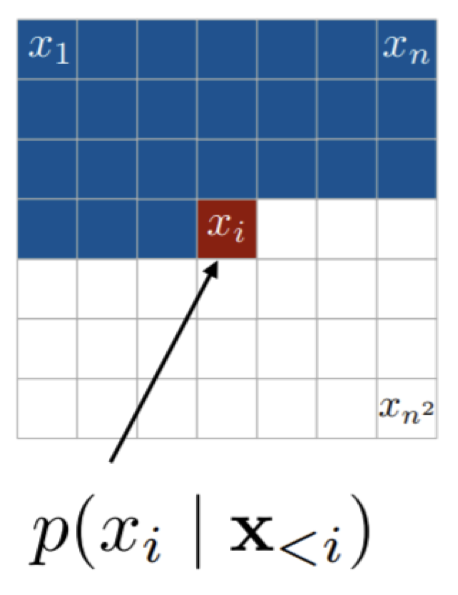
\includegraphics[width=0.3\columnwidth]{figures/pixelcnn.png}
%     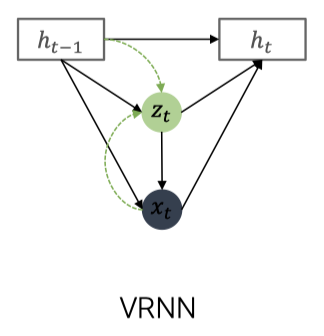
\includegraphics[width=0.4\columnwidth]{figures/VRNN.png}
% \end{center}

\subsection*{Temporal causal NN (TCN): WaveNet}

Idea: Adapt PixelCNN to Audio.

Prob: larger dim than images (\(>16000/{s}\)).

Trick: Dilated Conv, exponential increase in receptive field. (Stride Conv not allow to preserve resolution)

\subsection*{Variational RNN}

\textbf{Goal} increase expressiveness, noise robustness by stochastic latent variables into hidden state of an RNN.

\textbf{Model}
(1) Deterministic transition \(h_{t}=f_{\theta}(h_{t-1}, x_{t}, z_{t})\).
(2) Dynamic prior \(p_{\theta}(z_{t} | h_{t-1})\), overall prior \(p_{\theta}(z)=\prod_{t=1}^{T} p_{\theta}(z_{t}|z_{<t}, x_{<t}) = \prod_{t=1}^{T} p_{\theta}(z_{t} | h_{t-1})\times\) \( p_{f_\theta}(h_{t-1} | h_{t-2}, z_{t-1}, x_{t-1})\). Each $z_t$ depends on previous $x_{<t}$ and $z_{<t}$.

\textbf{Adv} for \(z\) in \(f_{\theta}\): (1) robust by randomness of \(z\) (2) latent \(z\) is high level, more informative on future.

\textbf{{Dec}}: \(p(x_{t} | z_{t})=g^{\text{out}}(h_{t-1}, z_{t})\),

\textbf{{Enc}}: \(q_{\phi}(z | x)=\prod_{t=1}^{T} q_{\phi}(z_{t} | x_{t}, x_{<t}, z_{<t})\),

\textbf{{ELBO}} \(\sum_t \log p_{\theta}(x_{t}|x_{< t}) \geq \mathcal{L}_{\theta, \phi}=\sum_{t=1}^{T} \mathbb{E}_{q_{\phi}(z_{t} | x_{t}, x_{<t}, z_{<t})}[\log p_{\theta}(x_{t} | z_{t}, z_{<t}, x_{<t})]-\KL(q_{\phi}(z_{t} | x_{t}, x_{<t}, z_{<t}) \| p_{\theta}(z_{t} | z_{<t}, x_{<t}))\).

KL in VRNN: (1) balance the informative \(z_t\) from \(x_t\) dependent \(q_\phi\) (if not \(x_t\) depend, \(z_t\) mostly from \(h_{t-1}\)) and overfit to memorize \(x_t\) by KL to prior. (2) Force the prior also to be informative from \(h_{t-1}\).


\subsection*{Conditional VRNN}

Hidden state \(\{z_t, \pi_t\}\).
Priors: \(p(z_{t} | h_{t-1})=g^{p, z}(h_{t-1})\), \( p(\pi_{t} | h_{t-1})=g^{p, \pi}(h_{t-1})\).
Transition: \(h_{t}=\tau(x_{t}, z_{t}, \pi_{t}, h_{t-1})\)
\textsf{{D}}: \(p(x_{t} | z_{t}, \pi_{t})=g^{\text {out}}(z_{t}, \pi_{t})\) (no \(h_{t-1}\) here).
\textsf{{E}}: \(q(z_{t} | x_{t})=g^{q, z}(h_{t-1}, x_{t}) \), \( q(\pi_{t} | x_{t})=g^{q, \pi}(h_{t-1}, x_{t})\).\\
\textsf{{ELBO}}: \( \sum_{t=1}^{T} \mathbb{E}_{q(z_{t}, \pi_{t}  x_{t})} \log p(x_{t}  z_{t}, \pi_{t})- \KL (q(z_{t}  x_{t}) \| p(z_{t})) - \KL(q(\pi_{t}  x_{t}) \| p(\pi_{t}))\)

\textbf{APP} Digital Handwriting Modeling.

\subsection*{Summary}
\textbf{Pros} \(p(x)\) tractable, explicit NLL metric to compare performance, easy to train, sample.
\textbf{Cons} Slow, no natural latent variable representation (except C-VRNN, STCN).
% \begin{center}
%     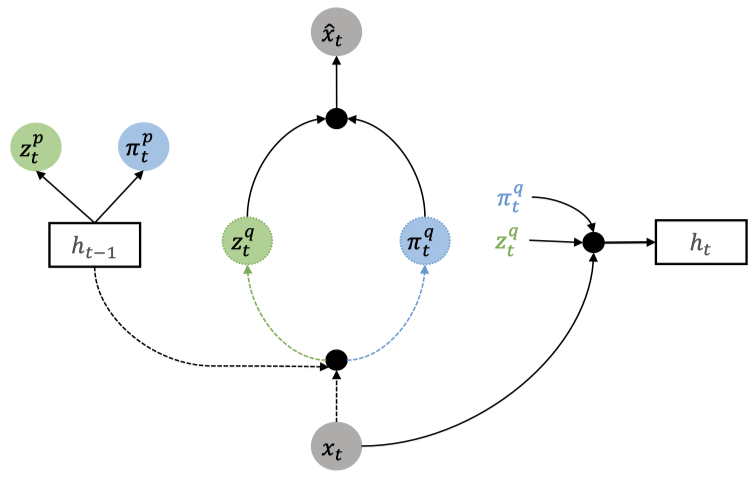
\includegraphics[width=0.7\columnwidth]{figures/C-VRNN.png}
% \end{center}

\subsection*{Self-attentioan and Transformers}

\(X=\operatorname{softmax}({({W}_{{Q}} {X})({W}_{{K}} {X})^{\top}}/{\sqrt{D}}+M) \odot {W}_{{V}} {X}\), mask \(M\) prevent accessing future. 

\textbf{Positional Encoding} unique sinusoidal encoding to preserve ordering. \(\mathsf{PE}_{i, t} =  \sin\text{/}\cos (\omega_{k} t)\) for \(i= 2k\text{/} 2k+1\), \(\omega_{k}=10000^{-{2 k}/{d}}\), \(t\) position in seq, \(i\) component in embedding vec.
Cost \(O(T^2 D)\).

\textbf{Trick} multi-head attention.

\textbf{APP} 3D human pose and mesh recon, 3D objects Mesh generation, 3D human motion modelling.

\subsection*{LLM / GPT}

Needs tokenization, can be finetuned by combining unsupervised pretraining $L_1(X) = \sum \log P(x_i|x_{i-1:i-k})$ plus supervised finetuning $L_2(X,Y) =$ $ \sum \log P(y|x\dots)$, then $L=L_2(X,Y) + \lambda L_1(X)$

For \textbf{autoreg. image/video generation}: problems with image quality, computational requirements. Solution: quantize images into tokens (e.g. Vector-Quantized \textbf{VQ-VAE} uses CNN enc/dec): lower dimensionality, more semantically meaningful. Also, can use LLMs.

% Application: 
% 3D human pose and mesh reconstruction: Conditioned on input image. Initializing 3D joints and 3D mesh vertex positions with T-pose. Refining 3D joints and 3D mesh vertices via self-attention. Randomly masking some joints and vertices to improve robustness., 


% Mesh generation for 3D objects: Given the current set of vertices V, estimates a predictive distribution for the next vertex coordinates z, y and x or a stopping token. \(p(\mathcal{V}^{{seq}} ; \theta)=\prod_{n=1}^{N_{V}} p(v_{n} | v_{<n} ; \theta)\), Similar to PixelCNN and WaveNet, 3D vertex coordinates are quantized and represented via discrete random var.

% The face model takes collection of vertices, as input a and the current sequence of face indices, and outputs a distribution over vertex indices. \(p(\mathcal{F}^{{seq}} | \mathcal{V} ; \theta)=\prod_{n=1}^{N_{F}} p(f_{n} | f_{<n}, \mathcal{V} ; \theta)\)


% 3D human motion modelling: Given a sequence of past frames, predicts the future. Decoupled attention over the temporal and spatial dimensions. To predict a joint in the next step, aggregates information from the past instances of the same joint and other joints at the current step.
